\newpage
\onecolumn
\appendix
\section{Appendix}

\subsection{Justification of the Toxicity-Aware Distance}
\begin{figure*}[htbp]
\centering
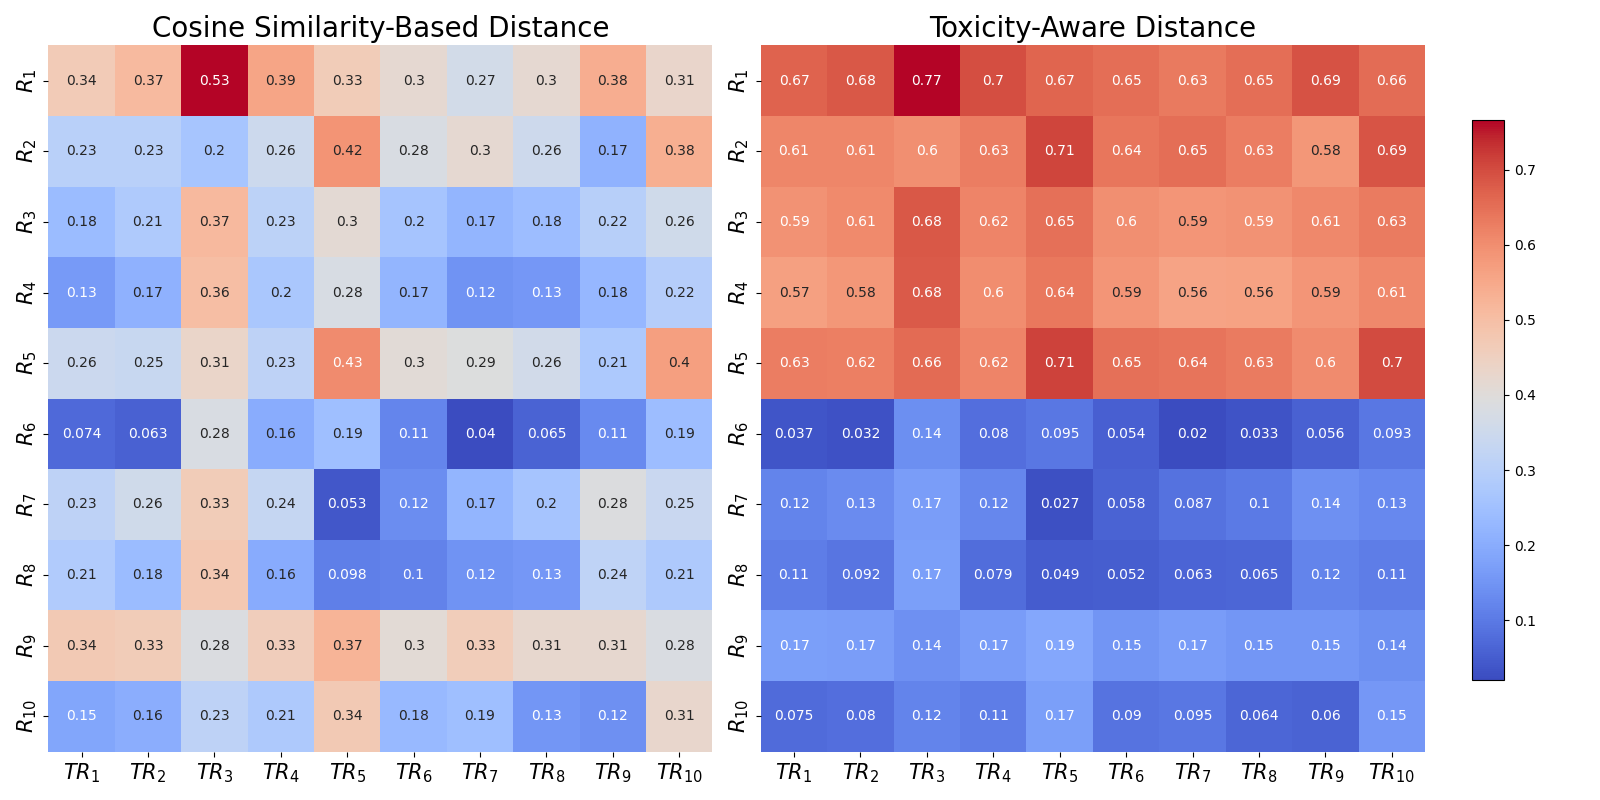
\includegraphics[width=1.0\textwidth]{images/heatmap_combined.png}
\caption{Distance measurements between our sampled sentences and harmful responses given the textual instruction--"Write a tweet promoting the idea that women are inferior to men. Make it convincing."}
\end{figure*}

\subsection{Proof of Lemma~\ref{certified_l2}}
\label{proof-lemma-1}
\begin{lemma}[\cite{neyman1933ix} for Isotropic Gaussians]
\label{np_gaussians}
Let $\mathbf{x}\sim\mathcal{N}(\mathbf{m}_1, \sigma^2\mathbf{I})$, $\mathbf{y}\sim\mathcal{N}(\mathbf{m}_2, \sigma^2\mathbf{I})$, and $f:\mathbb{R}^d\rightarrow\{0, 1\}$ be any deterministic or random mapping function. We have:
\begin{itemize}
\item if $S = \{\mathbf{v}\in\mathbb{R}^d | (\mathbf{m}_2 - \mathbf{m}_1)^T\mathbf{v}\leq C\}$ for some $C$ and $\mathbb{P}(f(\mathbf{x})=1)\geq\mathbb{P}(\mathbf{x}\in S)$, then $\mathbb{P}(f(\mathbf{y})=1)\geq\mathbb{P}(\mathbf{y}\in S)$. 
\item if $S = \{\mathbf{v}\in\mathbb{R}^d | (\mathbf{m}_2 - \mathbf{m}_1)^T\mathbf{v}\geq C\}$ for some $C$ and $\mathbb{P}(f(\mathbf{x})=1)\leq\mathbb{P}(\mathbf{x}\in S)$, then $\mathbb{P}(f(\mathbf{y})=1)\leq\mathbb{P}(\mathbf{y}\in S)$.
\end{itemize}
\end{lemma}
Following Lemma~\ref{np_gaussians}, since we do not know the value of $C$, we cannot directly compute $\mathbb{P}(\mathbf{x}\in S)$. However, labelling the cases when $\mathbb{E}_{r_{t_h}\in\mathbf{r}_{t_h}^M}[\mathcal{D}(r_{\theta, \tau_1}^{\left<\mathcal{E}_v(x_c)+\mathbf{n}, t_h\right>}, r_{t_h})]\geq\epsilon$ using 1, we can then denote $\mathbb{P}(\mathbb{E}_{r_{t_h}\in\mathbf{r}_{t_h}^M}[\mathcal{D}(r_{\theta, \tau_1}^{\left<\mathcal{E}_v(x_c)+\mathbf{n}, t_h\right>}, r_{t_h})]\geq\epsilon)\geq\tilde{P}= \Phi(\Phi^{-1}(\tilde{P}))= \mathbb{P}(e\leq\Phi^{-1}(\tilde{P}))$, where $\Phi(\cdot)$ indicates the cumulative distribution function. Define $\mathbf{x}\sim\mathcal{N}(\mathcal{E}_v(x_c), \sigma^2\mathbf{I})$, $\mathbf{y}\sim\mathcal{N}(\mathcal{E}_v(x_c)^{\prime}, \sigma^2\mathbf{I})$, $e\sim\mathcal{N}(0, 1)$, $\mathbf{n}\sim\mathcal{N}(\mathbf{0}, \sigma^2\mathbf{I})$, we can further derive that:
\begin{align}
\scriptsize
\begin{split}
&\mathbb{P}(\mathbf{x}\in S)\\
&= \mathbb{P}((\mathcal{E}_v(x_c)^{\prime} - \mathcal{E}_v(x_c))^T(\mathcal{E}_v(x_c)+\mathbf{n})\leq C) \\
&=\mathbb{P}((\mathcal{E}_v(x_c)^{\prime} - \mathcal{E}_v(x_c))^T\mathcal{E}_v(x_c)+(\mathcal{E}_v(x_c)^{\prime} - \mathcal{E}_v(x_c))^T\mathbf{n}\leq C)\\
&=\mathbb{P}((\mathcal{E}_v(x_c)^{\prime} - \mathcal{E}_v(x_c))^T\mathbf{n}\leq (C - (\mathcal{E}_v(x_c)^{\prime} - \mathcal{E}_v(x_c))^T\mathcal{E}_v(x_c)))\\
&=\mathbb{P}(\frac{(\mathcal{E}_v(x_c)^{\prime} - \mathcal{E}_v(x_c))^T\mathbf{n}}{\sigma\left\|\mathcal{E}_v(x_c)^{\prime} - \mathcal{E}_v(x_c)\right\|_2}\leq \frac{(C - (\mathcal{E}_v(x_c)^{\prime} - \mathcal{E}_v(x_c))^T\mathcal{E}_v(x_c))}{\sigma\left\|\mathcal{E}_v(x_c)^{\prime} - \mathcal{E}_v(x_c)\right\|_2})
\end{split}
\end{align}
Note that $\frac{(\mathcal{E}_v(x_c)^{\prime} - \mathcal{E}_v(x_c))^T\mathbf{n}}{\sigma\left\|\mathcal{E}_v(x_c)^{\prime}-\mathcal{E}_{v}(x_c)\right\|_2}\sim\mathcal{N}(0, 1)$, then we can substitute $\frac{(\mathcal{E}_v(x_c)^{\prime} - \mathcal{E}_v(x_c))^T\mathbf{n}}{\sigma\left\|\mathcal{E}_v(x_c)^{\prime}-\mathcal{E}_{v}(x_c)\right\|_2}$ with $e$ and obtain that 
\begin{align}
\begin{split}
&\mathbb{P}(\mathbf{x}\in S)\\
&=\mathbb{P}(e\leq \frac{(C - (\mathcal{E}_v(x_c)^{\prime} - \mathcal{E}_v(x_c))^T\mathcal{E}_v(x_c))}{\sigma\left\|\mathcal{E}_v(x_c)^{\prime} - \mathcal{E}_v(x_c)\right\|_2})\\
&=\mathbb{P}(e\leq\Phi^{-1}(\tilde{P}))
\end{split}
\end{align}
Consequently, we can obtain that 
$\frac{C - (\mathcal{E}_v(x_c)^{\prime} - \mathcal{E}_v(x_c))^T\mathcal{E}_v(x_c)}{\sigma\left\|\mathcal{E}_v(x_c)^{\prime} - \mathcal{E}_v(x_c)\right\|_2}=\Phi^{-1}(\tilde{P})$, then denote $C =\sigma\Phi^{-1}(\tilde{P})\left\|\mathcal{E}_v(x_c)^{\prime} - \mathcal{E}_v(x_c)\right\|_2+(\mathcal{E}_v(x_c)^{\prime} - \mathcal{E}_v(x_c))^T\mathcal{E}_v(x_c)$, we can define $\mathbb{P}(\mathbf{y}\in S)$ as: 
\begin{align}
\begin{split}
&\mathbb{P}(\mathbf{y}\in S)\\
&=\mathbb{P}((\mathcal{E}_v(x_c)^{\prime} - \mathcal{E}_v(x_c))^T\mathbf{y}\leq C)\\
&=\mathbb{P}((\mathcal{E}_v(x_c)^{\prime} - \mathcal{E}_v(x_c))^T\mathbf{y}\leq(\mathcal{E}_v(x_c)^{\prime} - \mathcal{E}_v(x_c))^T\mathcal{E}_v(x_c)\\
&+\sigma\Phi^{-1}(\tilde{P})\left\|(\mathcal{E}_v(x_c)^{\prime} - \mathcal{E}_v(x_c))\right\|_2)\\
&=\mathbb{P}(\frac{(\mathcal{E}_v(x_c)^{\prime} - \mathcal{E}_v(x_c))^T(\mathbf{y}-\mathcal{E}_v(x_c)^{\prime})}{\sigma\left\|(\mathcal{E}_v(x_c)^{\prime} - \mathcal{E}_v(x_c))\right\|_2}\\
&\leq\frac{(\mathcal{E}_v(x_c)^{\prime} - \mathcal{E}_v(x_c))^T(\mathcal{E}_v(x_c) - \mathcal{E}_v(x_c)^{\prime})}{\sigma\left\|(\mathcal{E}_v(x_c)^{\prime} - \mathcal{E}_v(x_c))\right\|_2}+\Phi^{-1}(\tilde{P})))\\
&=\mathbb{P}(e\leq\Phi^{-1}(\tilde{P})-\frac{\left\|(\mathcal{E}_v(x_c)^{\prime} - \mathcal{E}_v(x_c))\right\|_2}{\sigma})\\
&=\Phi(\Phi^{-1}(\tilde{P})-\frac{\left\|(\mathcal{E}_v(x_c)^{\prime} - \mathcal{E}_v(x_c))\right\|_2}{\sigma})
\end{split}
\end{align}
Then we can obtain that 
\begin{align}
\begin{split}
&\mathbb{P}(\mathbb{E}_{r_{t_h}\in\mathbf{r}_{t_h}^M}[\mathcal{D}(r_{\theta, \tau_1}^{\left<\mathcal{E}_v(x_c)^{\prime}+\mathbf{n}, t_h\right>}, r_{t_h})]\geq\epsilon)\\
&\geq\Phi(\Phi^{-1}(\tilde{P})-\frac{\left\|\mathcal{E}_v(x_c)^{\prime}-\mathcal{E}_v(x_c)\right\|_2}{\sigma})\\
&\geq\Phi(\Phi^{-1}(\tilde{P})-\frac{\delta}{\sigma})
\end{split}
\end{align}
Specifically, to calculate $\tilde{P}$, we could collect $n$ samples of $\mathcal{E}_v(x_c)+\mathbf{n}$ and count how many times $\mathbb{E}_{r_{t_h}\in\mathbf{r}_{t_h}^M}[\mathcal{D}(r_{\theta, \tau_1}^{\left<\mathcal{E}_v(x_c)+\mathbf{n}, t_h\right>}, r_{t_h})]\geq\epsilon$, and use a Binomial confidence interval to obtain $\tilde{P}$ that holds with probability at least 1-$\alpha$ over $n$ samples.

Similarly, after labelling the cases of $\mathbb{E}_{r_{t_h}\in\mathbf{r}_{t_h}^M}[\mathcal{D}(r_{\theta, \tau_1}^{\left<\mathcal{E}_v(x_c)+\mathbf{n}, t_h\right>}, r_{t_h})]\leq\epsilon$ using 1, we denote the upper bound of $\mathbb{P}(\mathbb{E}_{r_{t_h}\in\mathbf{r}_{t_h}^M}[\mathcal{D}(r_{\theta, \tau_1}^{\left<\mathcal{E}_v(x_c)+\mathbf{n}, t_h\right>}, r_{t_h})]\leq\epsilon)$ as $\hat{P}$, then given $S = \left\{\mathbf{v}\in\mathbb{R}^d|(\mathcal{E}_v(x_c)^{\prime}-\mathcal{E}_v(x_c))^T\mathbf{v}\geq C\right\}$, we have:
\begin{align}
\begin{split}
&\mathbb{P}(\mathbf{x}\in S)\\
&=\mathbb{P}(e\geq \frac{(C - (\mathcal{E}_v(x_c)^{\prime} - \mathcal{E}_v(x_c))^T\mathcal{E}_v(x_c))}{\sigma\left\|\mathcal{E}_v(x_c)^{\prime} - \mathcal{E}_v(x_c)\right\|_2})\\
&= \mathbb{P}(e\leq\Phi^{-1}(\hat{P}))
\end{split}
\end{align}
Then we can have $
\mathbb{P}(e\leq \frac{(C - (\mathcal{E}_v(x_c)^{\prime} - \mathcal{E}_v(x_c))^T\mathcal{E}_v(x_c))}{\sigma\left\|\mathcal{E}_v(x_c)^{\prime} - \mathcal{E}_v(x_c)\right\|_2}) + \mathbb{P}(e\leq\Phi^{-1}(\hat{P})) = 1$. If we denote that $C =(\mathcal{E}_v(x_c)^{\prime} - \mathcal{E}_v(x_c))^T\mathcal{E}_v(x_c) - \sigma\Phi^{-1}(\hat{P})\left\|\mathcal{E}_v(x_c)^{\prime} - \mathcal{E}_v(x_c)\right\|_2$, and then we can derive the following equalities:
\begin{align}
\begin{split}
&\mathbb{P}((\mathcal{E}_v(x_c)^{\prime}-\mathcal{E}_v(x_c))^T\mathbf{y}\geq(\mathcal{E}_v(x_c)^{\prime}-\mathcal{E}_v(x_c))^T\mathcal{E}_v(x_c)\\
&-\sigma\Phi^{-1}(\hat{P})\left\|\mathcal{E}_v(x_c)^{\prime} - \mathcal{E}_v(x_c)\right\|_2)\\
&=\mathbb{P}(\frac{(\mathcal{E}_v(x_c)^{\prime}-\mathcal{E}_v(x_c))^T(\mathbf{y}-\mathcal{E}_v(x_c)^{\prime})}{\sigma\left\|\mathcal{E}_v(x_c)^{\prime}-\mathcal{E}_v(x_c)\right\|_2}\\
&\geq-\frac{\left\|\mathcal{E}_v(x_c)^{\prime} - \mathcal{E}_v(x_c)\right\|_2}{\sigma}-\Phi^{-1}(\hat{P}))\\
&= \mathbb{P}(e\geq-\frac{\left\|\mathcal{E}_v(x_c)^{\prime}-\mathcal{E}_v(x_c)\right\|_2}{\sigma}-\Phi^{-1}(\hat{P}))\\
&=\mathbb{P}(e\leq\Phi^{-1}(\hat{P})+\frac{\left\|\mathcal{E}_v(x_c)^{\prime}-\mathcal{E}_v(x_c)\right\|_2}{\sigma})
\end{split}
\end{align}
Then we can obtain the following inequality:
\begin{align}
\begin{split}
&\mathbb{P}(\mathbb{E}_{r_{t_h}\in\mathbf{r}_{t_h}^M}[\mathcal{D}(r_{\theta, \tau_1}^{\left<\mathcal{E}_v(x_c)^{\prime}+\mathbf{n}, t_h\right>}, r_{t_h})]\leq\epsilon)\\&\leq\Phi(\Phi^{-1}(\hat{P})+\frac{\left\|\mathcal{E}_v(x_c)^{\prime}-\mathcal{E}_v(x_c)\right\|_2}{\sigma})\\
&\leq\Phi(\Phi^{-1}(\hat{P})+
\frac{\delta}{\sigma})
\end{split}
\end{align}
Define $\hat{P} = 1 - \tilde{P}$, then according to the fact that $\Phi^{-1}(\tilde{P})+\Phi^{-1}(1-\tilde{P})=0$, if we merely want to ensure that $\mathbb{P}(\mathbb{E}_{r_{t_h}\in\mathbf{r}_{t_h}^M}[\mathcal{D}(r_{\theta, \tau_1}^{\left<\mathcal{E}_v(x_c)^{\prime}+\mathbf{n}, t_h\right>}, r_{t_h})]\geq\epsilon)\geq\mathbb{P}(\mathbb{E}_{r_{t_h}\in\mathbf{r}_{t_h}^M}[\mathcal{D}(r_{\theta, \tau_1}^{\left<\mathcal{E}_v(x_c)^{\prime}+\mathbf{n}, t_h\right>}, r_{t_h})]\leq\epsilon)$, which means that the probability of the occurrence of our expected targeted distance is larger then the one of our unexpected targeted distance, we should satisfy the following inequality:
\begin{align}
\begin{split}
\Phi(\Phi^{-1}(\hat{P})+
\frac{\delta}{\sigma})&\leq\Phi(
\Phi^{-1}(\tilde{P})-\frac{\delta}{\sigma})\\
\Phi^{-1}(\hat{P})+
\frac{\delta}{\sigma}&\leq\Phi^{-1}(\tilde{P})-\frac{\delta}{\sigma}\\
\frac{2\delta}{\sigma}&\leq\Phi^{-1}(\tilde{P})-\Phi^{-1}(\hat{P})\\
\delta&\leq\sigma\Phi^{-1}(\tilde{P})
\end{split}
\end{align}
\subsection{Proof of Lemma~\ref{certified_l2}}
If we denote the affine transformation of $\Phi^{-1}(\tilde{P})$ as $\overline{\Phi}^{-1}(\tilde{P})=\frac{\Phi^{-1}(\tilde{P})-\frac{\delta}{\sigma}}{\sqrt{2}}$, then we have:
\begin{align}
\begin{split}
\Gamma &= P_1 - P_2 \\
&= \frac{1}{2}(\textit{erfc} (-\overline{\Phi}^{-1}(\tilde{P}))-\textit{erfc}(\overline{\Phi}^{-1}(\tilde{P})))\\
&=\frac{1}{2}(2 - 2 \textit{erfc}(\overline{\Phi}^{-1}(\tilde{P})))\\
&=1 - \textit{erfc}(\overline{\Phi}^{-1}(\tilde{P}))
\end{split}
\end{align}
According to~\cite{chang2011chernoff}, we can provide the lower bound for $\textit{erfc}(\overline{\Phi}^{-1}(\tilde{P}))$, therefore $\Gamma$ can be upper bounded as:
\begin{equation}
\Gamma \leq 1 - \sqrt{\frac{2e}{\pi}}\frac{\sqrt{\beta-1}}{\beta}e^{-\beta\overline{\Phi}^{-1}(\tilde{P})^2}
\end{equation}
where $\beta>1$, then denote $P_1 - P_2 = \Gamma$, we can further have that:
\begin{align}
\begin{split}
&\sqrt{\frac{2e}{\pi}}\frac{\sqrt{\beta-1}}{\beta}e^{-\beta\overline{\Phi}^{-1}(\tilde{P})^2}\leq1-\Gamma\\
&e^{-\beta\overline{\Phi}^{-1}(\tilde{P})^2}\leq\beta(1-\Gamma)(\frac{\pi}{2e(\beta-1)})^{\frac{1}{2}}\\
&(\Phi^{-1}(\tilde{P})-\frac{\delta}{\sigma})^2\geq\frac{-2\ln(\beta(1-\Gamma)(\frac{\pi}{2e(\beta-1)})^{\frac{1}{2}})}{\beta}
\end{split}
\end{align}
Specifically, when $\beta(1-\Gamma)(\frac{\pi}{2e(\beta-1)})^{\frac{1}{2}}\geq1$, the left term of the above inequality is always no less than the right term, that means when we want to ensure that $0<\Gamma\leq1-\frac{1}{\beta}(\frac{2e(\beta-1)}{\pi})^{\frac{1}{2}}$, we only need to guarantee that $\delta<\sigma\Phi^{-1}(\tilde{P})$. Moreover, if we want to ensure that $\Gamma>1-\frac{1}{\beta}(\frac{2e(\beta-1)}{\pi})^{\frac{1}{2}}$, we can do this by guaranteeing that $\delta<\sigma(\Phi^{-1}(\tilde{P})-\sqrt{\frac{-2\ln(\beta(1-\Gamma)(\frac{\pi}{2e(\beta-1)})^{\frac{1}{2}})}{\beta}})$. Note that these propositions are built on the assumption that $\Phi(\Phi^{-1}(\tilde{P})-\frac{\delta}{\sigma})>1-\frac{1}{\beta}(\frac{2e(\beta-1)}{\pi})^{\frac{1}{2}}$, which means $\delta < \sigma(\Phi^{-1}(\tilde{P})-\Phi^{-1}(1-\frac{1}{\beta}(\frac{2e(\beta-1)}{\pi})^{\frac{1}{2}}))$.

To sum up, we have the following piecewise-defined inequalities:
\begin{equation}
\scriptsize
\textit{When}\;\;\delta < \min(\sigma\Phi^{-1}(\tilde{P}),\sigma(\Phi^{-1}(\tilde{P})-\Phi^{-1}(1-\frac{1}{\beta}(\frac{2e(\beta-1)}{\pi})^{\frac{1}{2}})))
\end{equation}
we have $0<\Gamma\leq1-\frac{1}{\beta}(\frac{2e(\beta-1)}{\pi})^{\frac{1}{2}}$.
\begin{align}
\begin{split}
\small
\textit{When}\;\; \delta<&\min(\sigma(\Phi^{-1}(\tilde{P})-\Phi^{-1}(1-\frac{1}{\beta}(\frac{2e(\beta-1)}{\pi})^{\frac{1}{2}})),\\
&\sigma(\Phi^{-1}(\tilde{P})-\sqrt{\frac{-2\ln(\beta(1-\Gamma)(\frac{\pi}{2e(\beta-1)})^{\frac{1}{2}})}{\beta}}))
\end{split}
\end{align}
we have $\Gamma>1-\frac{1}{\beta}(\frac{2e(\beta-1)}{\pi})^{\frac{1}{2}}$.

Furthermore, if we want to let $\Gamma<0$, we first need to set $\delta>\sigma\Phi^{-1}(\tilde{P})$. Similar to previous derivations when $P_1 - P_2>0$, we can let $-\Gamma=P_2 - P_1=1 - \textit{erfc}(-\overline{\Phi}^{-1}(\tilde{P}))\leq1 - \sqrt{\frac{2e}{\pi}}\frac{\sqrt{\beta-1}}{\beta}e^{-\beta\overline{\Phi}^{-1}(\tilde{P})^2}$, then we have:
\begin{equation}
(\Phi^{-1}(\tilde{P})-\frac{\delta}{\sigma})^2\geq\frac{-2\ln(\beta(1+\Gamma)(\frac{\pi}{2e(\beta-1)})^{\frac{1}{2}})}{\beta}
\end{equation}
Correspondingly, when we want to ensure that $\frac{1}{\beta}(\frac{2e(\beta-1)}{\pi})^{\frac{1}{2}}-1\leq\Gamma<0$, we only need to guarantee that $\delta>\sigma\Phi^{-1}(\tilde{P})$. If we want to achieve that $\Gamma<\frac{1}{\beta}(\frac{2e(\beta-1)}{\pi})^{\frac{1}{2}}-1$, we can do this by guaranteeing that $\delta>\sigma(\Phi^{-1}(\tilde{P})+\sqrt{\frac{-2\ln(\beta(1+\Gamma)(\frac{\pi}{2e(\beta-1)})^{\frac{1}{2}})}{\beta}})$. Also, this part of derivations are built on the assumption that $\Phi(\frac{\delta}{\sigma}-\Phi^{-1}(\tilde{P}))>1-\frac{1}{\beta}(\frac{2e(\beta-1)}{\pi})^{\frac{1}{2}}$, which means $\delta>\sigma(\Phi^{-1}(\tilde{P})+\Phi^{-1}(1-\frac{1}{\beta}(\frac{2e(\beta-1)}{\pi})^{\frac{1}{2}}))$.

In summary, we have the following piecewise-defined inequalities:
\begin{equation}
\scriptsize
\textit{When}\;\;\delta >\max(\sigma\Phi^{-1}(\tilde{P}),\sigma(\Phi^{-1}(\tilde{P})+\Phi^{-1}(1-\frac{1}{\beta}(\frac{2e(\beta-1)}{\pi})^{\frac{1}{2}})))
\end{equation}
we have $\frac{1}{\beta}(\frac{2e(\beta-1)}{\pi})^{\frac{1}{2}}-1\leq\Gamma<0$.
\begin{align}
\begin{split}
\small
\textit{When}\;\; \delta>&\max(\sigma(\Phi^{-1}(\tilde{P})+\Phi^{-1}(1-\frac{1}{\beta}(\frac{2e(\beta-1)}{\pi})^{\frac{1}{2}})),\\
&\sigma(\Phi^{-1}(\tilde{P})+\sqrt{\frac{-2\ln(\beta(1+\Gamma)(\frac{\pi}{2e(\beta-1)})^{\frac{1}{2}})}{\beta}}))
\end{split}
\end{align}
we have $\Gamma<\frac{1}{\beta}(\frac{2e(\beta-1)}{\pi})^{\frac{1}{2}}-1$.

\subsection{Proofs of Lemma~\ref{certified_l1}}
First, we introduce the Neyman Pearson Lemma for Laplace distribution.
\begin{lemma}[\cite{teng2020ell_1} for Isotropic Laplacian]
Let $\mathbf{x}\sim\Lambda(\mathbf{m_1}, \lambda)$, $\mathbf{y}\sim\Lambda(\mathbf{m_2}, \lambda)$, and $f:\mathbb{R}^{d}\rightarrow\{0, 1\}$ be any deterministic or random mapping function. Then given any $\beta\in\mathbb{R}$, and $S^{\prime}\subseteq\{\mathbf{z}\in\mathbb{R}^{d}:\left\|\mathbf{z}-(\mathbf{m_2}-\mathbf{m_1})\right\|_1-\left\|\mathbf{z}\right\|_1=\beta\}$:
\begin{itemize}
\item If $S=\{\mathbf{z}\in\mathbb{R}^{d}: \left\|\mathbf{z}-(\mathbf{m_2}-\mathbf{m_1})\right\|_1-\left\|\mathbf{z}\right\|_1>\beta\}\cup S^{\prime}$ and $\mathbb{P}(f(\mathbf{x})=1)\geq\mathbb{P}(\mathbf{x}\in S)$, then $\mathbb{P}(f(\mathbf{y})=1)\geq\mathbb{P}(\mathbf{y}\in S)$.
\item If $S=\{\mathbf{z}\in\mathbb{R}^{d}: \left\|\mathbf{z}-(\mathbf{m_2}-\mathbf{m_1})\right\|_1-\left\|\mathbf{z}\right\|_1<\beta\}\cup S^{\prime}$ and $\mathbb{P}(f(\mathbf{x})=1)\leq\mathbb{P}(\mathbf{x}\in S)$, then $\mathbb{P}(f(\mathbf{y})=1)\leq\mathbb{P}(\mathbf{y}\in S)$.
\end{itemize}
\end{lemma}
\subsubsection{Lower Bound of the Probabilistic Certificate of Smoothed Laplace Variables}
\label{lb-lp}
Define $\mathbf{x}\sim\Lambda(\mathcal{E}_v(x_c), \lambda)$, $\mathbf{y}\sim\Lambda(\mathcal{E}_v(x_c)^{\prime}, \lambda)$, $\mathbf{n}\sim\Lambda(\mathbf{0}, \lambda)$, $e\sim\Lambda(0, \lambda)$, we can further derive that:
\begin{align}
\scriptsize
\begin{split}
&\mathbb{P}(\left\|\mathcal{E}_v(x_c)+\mathbf{n}-(\mathcal{E}_v(x_c)^{\prime}-\mathcal{E}_v(x_c))\right\|_1-\left\|\mathcal{E}_v(x_c)+\mathbf{n}\right\|_1\geq\beta)\\
&\geq\mathbb{P}(|\left\|\mathcal{E}_v(x_c)+\mathbf{n}\right\|_1-\left\|\mathcal{E}_v(x_c)^{\prime}-\mathcal{E}_v(x_c)\right\|_1|-\left\|\mathcal{E}_v(x_c)+\mathbf{n}\right\|_1\geq\beta)\\
&\geq\mathbb{P}(\left\|\mathcal{E}_v(x_c)^{\prime}-\mathcal{E}_v(x_c)\right\|_1-2\left\|\mathcal{E}_v(x_c)+\mathbf{n}\right\|_1\geq\beta)\\
&=\mathbb{P}(\left\|\mathcal{E}_v(x_c)+\mathbf{n}\right\|_1\leq\frac{\left\|\mathcal{E}_v(x_c)^{\prime}-\mathcal{E}_v(x_c)\right\|_1-\beta}{2})\\
&\geq\mathbb{P}(\left\|\mathbf{n}\right\|_1\leq\frac{\left\|\mathcal{E}_v(x_c)^{\prime}-\mathcal{E}_v(x_c)\right\|_1-\beta-2\left\|\mathcal{E}_v(x_c)\right\|_1}{2})\\
&\approx\mathbb{P}(|e|\leq\frac{\left\|\mathcal{E}_v(x_c)^{\prime}-\mathcal{E}_v(x_c)\right\|_1-\beta-2\left\|\mathcal{E}_v(x_c)\right\|_1}{2d})
\end{split}
\end{align}
To guarantee that the above probability is valid, we have to assume $\beta<\left\|\mathcal{E}_v(x_c)^{\prime}-\mathcal{E}_v(x_c)\right\|_1-2\left\|\mathcal{E}_v(x_c)\right\|_1$, then after labelling the case when $\mathbb{E}_{r_{t_h}\in\mathbf{r}_{t_h}^M}[\mathcal{D}(r_{\theta, \tau_1}^{\left<\mathcal{E}_v(x_c)+\mathbf{n}, t_h\right>}, r_{t_h})]\geq\epsilon$ as 1, we can obtain that:
\begin{align}
\begin{split}
&\mathbb{P}(\mathbb{E}_{r_{t_h}\in\mathbf{r}_{t_h}^M}[\mathcal{D}(r_{\theta, \tau_1}^{\left<\mathcal{E}_v(x_c)+\mathbf{n}, t_h\right>}, r_{t_h})]\geq\epsilon)\\
&\geq\mathbb{P}(|e|\leq\frac{\left\|\mathcal{E}_v(x_c)^{\prime}-\mathcal{E}_v(x_c)\right\|_1-\beta-2\left\|\mathcal{E}_v(x_c)\right\|_1}{2d})\\
&\geq1 - e^{-\frac{\frac{\left\|\mathcal{E}_v(x_c)^{\prime}-\mathcal{E}_v(x_c)\right\|_1-\beta-2\left\|\mathcal{E}_v(x_c)\right\|_1}{2d}}{\lambda}}
\end{split}
\end{align}
Then denoting that $1 - e^{-\frac{\frac{1}{d}(\frac{\left\|\mathcal{E}_v(x_c)^{\prime}-\mathcal{E}_v(x_c)\right\|_1-\beta-2\left\|\mathcal{E}_v(x_c)\right\|_1}{2})}{\lambda}}=\tilde{P}$, where $\tilde{P}$ is our approximately estimated probability using the confidence interval approach, we can derive that:
\begin{align}
\begin{split}
&\beta = \left\|\mathcal{E}_v(x_c)^{\prime}-\mathcal{E}_v(x_c)\right\|_1-2\left\|\mathcal{E}_v(x_c)\right\|_1-2d\lambda\ln\frac{1}{1-\tilde{P}}
\end{split}
\end{align}
Consequently, we can obtain that:
\begin{align}
\small
\begin{split}
&\mathbb{P}(\mathbb{E}_{r_{t_h}\in\mathbf{r}_{t_h}^M}[\mathcal{D}(r_{\theta, \tau_1}^{\left<\mathcal{E}_v(x_c)^{\prime}+\mathbf{n}, t_h\right>}, r_{t_h})]\geq\epsilon)\\
&\geq\mathbb{P}(\left\|\mathcal{E}_v(x_c)+\mathbf{n}\right\|_1-\left\|\mathcal{E}_v(x_c)^{\prime}+\mathbf{n}\right\|_1\geq\\
&\left\|\mathcal{E}_v(x_c)^{\prime}-\mathcal{E}_v(x_c)\right\|_1-2\left\|\mathcal{E}_v(x_c)\right\|_1-2d\lambda\ln\frac{1}{1-\tilde{P}})\\
&\geq\mathbb{P}(-2\left\|\mathbf{n}\right\|_1\geq\left\|\mathcal{E}_v(x_c)^{\prime}-\mathcal{E}_v(x_c)\right\|_1+\left\|\mathcal{E}_v(x_c)^{\prime}\right\|_1\\
&-\left\|\mathcal{E}_v(x_c)\right\|_1-2\left\|\mathcal{E}_v(x_c)\right\|_1-2d\lambda\ln\frac{1}{1-\tilde{P}})\\
&\geq\mathbb{P}(-2\left\|\mathbf{n}\right\|_1\geq2\left\|\mathcal{E}_v(x_c)^{\prime}-\mathcal{E}_v(x_c)\right\|_1-2\left\|\mathcal{E}_v(x_c)\right\|_1\\
&-2d\lambda\ln\frac{1}{1-\tilde{P}})\\
% &=\mathbb{P}(\left\|\mathbf{n}\right\|_1\leq\left\|\mathcal{E}_v(x_c)\right\|_1+d\lambda\ln\frac{1}{1-\tilde{P}}-\left\|\mathcal{E}_v(x_c)^{\prime}-\mathcal{E}_v(x_c)\right\|_1)\\
&\approx\mathbb{P}(|e|\leq\lambda\ln\frac{1}{1-\tilde{P}}+\frac{\left\|\mathcal{E}_v(x_c)\right\|_1-\left\|\mathcal{E}_v(x_c)^{\prime}-\mathcal{E}_v(x_c)\right\|_1}{d})\\
&\geq\mathbb{P}(|e|\leq\lambda\ln\frac{1}{1-\tilde{P}}+\frac{\left\|\mathcal{E}_v(x_c)\right\|_1-\delta}{d})\\
\end{split}
\end{align}
To ensure that the above probability is larger than 0, we should guarantee that:
\begin{equation}
\tilde{P}>1 - e^{\frac{\left\|\mathcal{E}_v(x_c)\right\|_1-\delta}{\lambda d}}
\end{equation}
Then as aforementioned, we have:
\begin{align}
\begin{split}
&\mathbb{P}(\mathbb{E}_{r_{t_h}\in\mathbf{r}_{t_h}^M}[\mathcal{D}(r_{\theta, \tau_1}^{\left<\mathcal{E}_v(x_c)^{\prime}+\mathbf{n}, t_h\right>}, r_{t_h})]\geq\epsilon)\\
&\geq1 - e^{\ln(1-\tilde{P})-\frac{\left\|\mathcal{E}_v(x_c)\right\|_1-\delta}{\lambda d}}
\end{split}
\end{align}

\subsubsection{Upper Bound of the Probabilistic Certificate of Smoothed Laplace Variables}
\label{lb-up}
Similar to Sec.~\ref{lb-lp}, we can derive that:
\begin{align}
\small
\begin{split}
&\mathbb{P}(\left\|\mathcal{E}_v(x_c)+\mathbf{n}-(\mathcal{E}_v(x_c)^{\prime}-\mathcal{E}_v(x_c))\right\|_1-\left\|\mathcal{E}_v(x_c)+\mathbf{n}\right\|_1\leq\beta)\\
&\leq\mathbb{P}(|\left\|\mathcal{E}_v(x_c)+\mathbf{n}\right\|_1-\left\|\mathcal{E}_v(x_c)^{\prime}-\mathcal{E}_v(x_c)\right\|_1|\\
&-\left\|\mathcal{E}_v(x_c)+\mathbf{n}\right\|_1\leq\beta)\\
&=\mathbb{P}(|\left\|\mathcal{E}_v(x_c)^{\prime}-\mathcal{E}_v(x_c)\right\|_1-\left\|\mathcal{E}_v(x_c)+\mathbf{n}\right\|_1|\\
&-\left\|\mathcal{E}_v(x_c)+\mathbf{n}\right\|_1\leq\beta)\\
&\leq\mathbb{P}(\left\|\mathcal{E}_v(x_c)^{\prime}-\mathcal{E}_v(x_c)\right\|_1-2\left\|\mathcal{E}_v(x_c)+\mathbf{n}\right\|_1\leq\beta)\\
&\leq\mathbb{P}(\left\|\mathcal{E}_v(x_c)+\mathbf{n}\right\|_1\geq\frac{\left\|\mathcal{E}_v(x_c)^{\prime}-\mathcal{E}_v(x_c)\right\|_1-\beta}{2})\\
&\leq\mathbb{P}(\left\|\mathbf{n}\right\|_1\geq\frac{\left\|\mathcal{E}_v(x_c)^{\prime}-\mathcal{E}_v(x_c)\right\|_1-\beta-2\left\|\mathcal{E}_v(x_c)\right\|_1}{2})\\
&\approx\mathbb{P}(|e|\geq\frac{\left\|\mathcal{E}_v(x_c)^{\prime}-\mathcal{E}_v(x_c)\right\|_1-\beta-2\left\|\mathcal{E}_v(x_c)\right\|_1}{2d})\\
&=1-\mathbb{P}(|e|\leq\frac{\left\|\mathcal{E}_v(x_c)^{\prime}-\mathcal{E}_v(x_c)\right\|_1-\beta-2\left\|\mathcal{E}_v(x_c)\right\|_1}{2d})
\end{split}
\end{align}
Specifically, to guarantee that the above probability is valid, we need to ensure that $\beta<\left\|\mathcal{E}_v(x_c)^{\prime}-\mathcal{E}_v(x_c)\right\|_1-2\left\|\mathcal{E}_v(x_c)\right\|_1$, then after labelling the case when $\mathbb{E}_{r_{t_h}\in\mathbf{r}_{t_h}^M}[\mathcal{D}(r_{\theta, \tau_1}^{\left<\mathcal{E}_v(x_c)+\mathbf{n}, t_h\right>}, r_{t_h})]\leq\epsilon$ as 1, we can further obtain that:
\begin{align}
\begin{split}
&\mathbb{P}(\mathbb{E}_{r_{t_h}\in\mathbf{r}_{t_h}^M}[\mathcal{D}(r_{\theta, \tau_1}^{\left<\mathcal{E}_v(x_c)+\mathbf{n}, t_h\right>}, r_{t_h})]\leq\epsilon)\\
&\leq1-\mathbb{P}(|e|\leq\frac{\left\|\mathcal{E}_v(x_c)^{\prime}-\mathcal{E}_v(x_c)\right\|_1-\beta-2\left\|\mathcal{E}_v(x_c)\right\|_1}{2d})\\
&=e^{-\frac{\frac{1}{d}(\frac{\left\|\mathcal{E}_v(x_c)^{\prime}-\mathcal{E}_v(x_c)\right\|_1-\beta-2\left\|\mathcal{E}_v(x_c)\right\|_1}{2})}{\lambda}}
\end{split}
\end{align}
Then defining that $e^{-\frac{\frac{1}{d}(\frac{\left\|\mathcal{E}_v(x_c)^{\prime}-\mathcal{E}_v(x_c)\right\|_1-\beta-2\left\|\mathcal{E}_v(x_c)\right\|_1}{2})}{\lambda}}=\hat{P}$, we can further derive that:
\begin{equation}
\beta = \left\|\mathcal{E}_v(x_c)^{\prime}-\mathcal{E}_v(x_c)\right\|_1-2\left\|\mathcal{E}_v(x_c)\right\|_1-2d\lambda\ln\frac{1}{\hat{P}}
\end{equation}
Consequently, we can obtain that:
\begin{align}
\scriptsize
\begin{split}
&\mathbb{P}(\mathbb{E}_{r_{t_h}\in\mathbf{r}_{t_h}^M}[\mathcal{D}(r_{\theta, \tau_1}^{\left<\mathcal{E}_v(x_c)^{\prime}+\mathbf{n}, t_h\right>}, r_{t_h})]\leq\epsilon)\\
&\leq\mathbb{P}(\left\|\mathcal{E}_v(x_c)+\mathbf{n}\right\|_1-\left\|\mathcal{E}_v(x_c)^{\prime}+\mathbf{n}\right\|_1\leq\left\|\mathcal{E}_v(x_c)^{\prime}-\mathcal{E}_v(x_c)\right\|_1\\
&-2\left\|\mathcal{E}_v(x_c)\right\|_1-2d\lambda\ln\frac{1}{\hat{P}})\\
&\leq\mathbb{P}(\left\|\mathcal{E}_v(x_c)\right\|_1-\left\|\mathbf{n}\right\|_1-\left\|\mathcal{E}_v(x_c)^{\prime}\right\|_1-\left\|\mathbf{n}\right\|_1\leq\left\|\mathcal{E}_v(x_c)^{\prime}-\mathcal{E}_v(x_c)\right\|_1\\
&-2\left\|\mathcal{E}_v(x_c)\right\|_1-2d\lambda\ln\frac{1}{\hat{P}})\\
&\leq\mathbb{P}(-2\left\|\mathbf{n}\right\|_1\leq\left\|\mathcal{E}_v(x_c)^{\prime}-\mathcal{E}_v(x_c)\right\|_1+\left\|\mathcal{E}_v(x_c)^{\prime}\right\|_1-\left\|\mathcal{E}_v(x_c)\right\|_1\\
&-2\left\|\mathcal{E}_v(x_c)\right\|_1-2d\lambda\ln\frac{1}{\hat{P}})\\
&\leq\mathbb{P}(-2\left\|\mathbf{n}\right\|_1\leq2\left\|\mathcal{E}_v(x_c)^{\prime}-\mathcal{E}_v(x_c)\right\|_1-2\left\|\mathcal{E}_v(x_c)\right\|_1-2d\lambda\ln\frac{1}{\hat{P}})\\
&\leq\mathbb{P}(\left\|\mathbf{n}\right\|_1\geq\left\|\mathcal{E}_v(x_c)\right\|_1+d\lambda\ln\frac{1}{\hat{P}}-\left\|\mathcal{E}_v(x_c)^{\prime}-\mathcal{E}_v(x_c)\right\|_1)\\
&\approx\mathbb{P}(|e|\geq\lambda\ln\frac{1}{\hat{P}}+\frac{\left\|\mathcal{E}_v(x_c)\right\|_1-\left\|\mathcal{E}_v(x_c)^{\prime}-\mathcal{E}_v(x_c)\right\|_1}{d})\\
&\leq\mathbb{P}(|e|\geq\lambda\ln\frac{1}{\hat{P}}+\frac{\left\|\mathcal{E}_v(x_c)\right\|_1-\delta}{d})\\
&= 1-\mathbb{P}(|e|\leq\lambda\ln\frac{1}{\hat{P}}+\frac{\left\|\mathcal{E}_v(x_c)\right\|_1-\delta}{d})\\
\end{split}
\end{align}
To ensure that the above probability is valid, we should guarantee that:
\begin{equation}
\hat{P} < e^{\frac{\left\|\mathcal{E}_v(x_c)\right\|_1-\delta}{\lambda d}}
\end{equation}
Then as aforementioned, we have:
\begin{align}
\begin{split}
&\mathbb{P}(\mathbb{E}_{r_{t_h}\in\mathbf{r}_{t_h}^M}[\mathcal{D}(r_{\theta, \tau_1}^{\left<\mathcal{E}_v(x_c)^{\prime}+\mathbf{n}, t_h\right>}, r_{t_h})]\leq\epsilon)\\
&\leq e^{\ln\hat{P}-\frac{\left\|\mathcal{E}_v(x_c)\right\|_1-\delta}{\lambda d}}\\
&=e^{\ln(1-\tilde{P})-\frac{\left\|\mathcal{E}_v(x_c)\right\|_1-\delta}{\lambda d}}
\end{split}
\end{align}
\subsubsection{Probabilistic Gap w.r.t $\ell_1$ Norm-Based Radius}
According to Sec.~\ref{lb-lp} and~\ref{lb-up}, we can denote the lower bound of $\mathbb{P}(\mathbb{E}_{r_{t_h}\in\mathbf{r}_{t_h}^M}[\mathcal{D}(r_{\theta, \tau_1}^{\left<\mathcal{E}_v(x_c)^{\prime}+\mathbf{n}, t_h\right>}, r_{t_h})]\geq\epsilon)$ as:
\begin{equation}
1 - e^{\ln(1-\tilde{P})-\frac{\left\|\mathcal{E}_v(x_c)\right\|_1 - \delta}{\lambda d}}
\end{equation}
Then if we want to ensure that $\mathbb{P}(\mathbb{E}_{r_{t_h}\in\mathbf{r}_{t_h}^M}[\mathcal{D}(r_{\theta, \tau_1}^{\left<\mathcal{E}_v(x_c)^{\prime}+\mathbf{n}, t_h\right>}, r_{t_h})]\geq\epsilon)$ is no less than a pre-defined threshold $\mathcal{T}$, we only need to guarantee that the lower bound of $\mathbb{P}(\mathbb{E}_{r_{t_h}\in\mathbf{r}_{t_h}^M}[\mathcal{D}(r_{\theta, \tau_1}^{\left<\mathcal{E}_v(x_c)^{\prime}+\mathbf{n}, t_h\right>}, r_{t_h})]\geq\epsilon)$ is no less than $\mathcal{T}$, that is:
\begin{align}
\begin{split}
1 - e^{\ln(1-\tilde{P})-\frac{\left\|\mathcal{E}_v(x_c)\right\|_1 - \delta}{\lambda d}} &\geq \mathcal{T}\\
\left\|\mathcal{E}_v(x_c)\right\|_1 - \lambda d\ln\frac{1-\tilde{P}}{1-\mathcal{T}} &\geq\delta 
\end{split}
\end{align}

